\section{Лекция 2}

\subsection{Формализация $\lambda$-термов, классы $\alpha$-эквивалентности термов}

\begin{definition}[$\lambda$-терм]
	Рассмотрим классы эквивалентности $[A]_{=_{\alpha}}$. \\
	Будем говорить, что $[A]\to_{\beta}[B]$, если существуют $A^{'}\in [A]$ и $B^{'} \in [B]$, что $A^{'}\to_{\beta}B^{'}$.
\end{definition}

\begin{lemma}
	$(=_{\alpha})$ "--- отношение эквивалентности.
\end{lemma}

Пусть в A есть $\beta$-редекc $(\lambda{}x.P)Q$, но $Q$ не свободен для подстановки вместо $x$ в $P$,
тогда найдем $y\notin V[P]$, $y\notin V[Q]$. Сделаем замену $P[x\coloneqq{}y]$.
Тогда замена $P[x\coloneqq{}y][y\coloneqq{}Q]$ допустима. То есть, можно сказать, что мы просто переименовали переменную $x$ в $P$ и получили свободу для подстановки, тем самым получив возможность редукции.

\begin{lemma}
	$P[x\coloneqq{}Q]=_{\alpha}P[x\coloneqq{}y][y\coloneqq{}Q]$, если замена допустима.
\end{lemma}

\subsection{Нормальная форма, $\lambda$-выражения без нормальной формы, \\комбинаторы $K$, $I$, $\Omega$}

\begin{definition}
	$\lambda$-выражение $A$ находится в нормальной форме, если оно не содержит $\beta$-редексов.
\end{definition}

\begin{definition}
	$A$ "--- нормальная форма $B$, если существует последовательность термов $A_{1} \dots A_{n}$ такая, что $B=_{\alpha}A_{1}\to_{\beta}A_{2}\to_{\beta}...\to_{\beta}A_{n}=_{\alpha}A$.
\end{definition}

\begin{definition}
	Комбинатор "--- $\lambda$-выражение без свободных переменных.
\end{definition}

\begin{definition} 
	\hfill
	\begin{itemize}
		\item $I \equiv \lambda{}x.x$ (Identitant)
		\item $K \equiv \lambda{}a.\lambda{}b.a$ (Konstanz)
		\item $\Omega \equiv (\lambda{}x.xx)(\lambda{}x.xx)$
	\end{itemize}
\end{definition}

\begin{lemma}
	$\Omega$ "--- не имеет нормальной формы.
\end{lemma}

\begin{proof}
	$\Omega$ имеет единственный $\beta$-редекс, где $A \equiv xx$, $B \equiv (\lambda{}x.xx)$. Тогда единственный возможный путь редукции "--- подставить $B$ вместо $x$ в $A$. Но тогда мы получим $\Omega$. Следовательно, у $\Omega$ нет нормальной формы, так как в полученном выражении у нас всегда будет $\beta$-редекс.
\end{proof}

\subsection{$\beta$-редуцируемость}

\begin{definition}
	Будем говорить, что $A\twoheadrightarrow_{\beta}B$, если $\exists$ такие $X_{1}$\ldots $X_{n}$, что $A=_{\alpha}X_{1}\to_{\beta}X_{2}\to_{\beta}\ldots\to_{\beta}X_{n-1}\to_{\beta}X_{n}=_{\alpha}B$.
\end{definition}

$(\twoheadrightarrow_{\beta})$ "--- рефлексивное и транзитивное замыкание $(\to_{\beta})$. $(\twoheadrightarrow_{\beta})$ не обязательно приводит к нормальной форме
\begin{example}
	$\Omega\twoheadrightarrow_{\beta}\Omega$
\end{example}

\subsection{Ромбовидное свойство}

\begin{definition}[Ромбовидное свойство]
	Отношение $R$ обладает ромбовидным свойством, если для любых $a,b,c$ таких, что $aRb$, $aRc$, $b\neq{}c$, существует $d$, что $bRd$ и $cRd$.
\end{definition}

\begin{example}
	$(\leq)$ на множестве натуральных чисел обладает ромбовидным свойством,
	$(>)$ на множестве натуральных чисел не обладает ромбовидным свойством.
\end{example}

\subsection{Теорема Чёрча-Россера, следствие о единственности \\нормальной формы}

\begin{theorem}[Черча-Россера]
	$(\twoheadrightarrow_{\beta})$ обладает ромбовидным свойством.
\end{theorem}


\begin{cons}
	Если у $A$ есть нормальная форма, то она единственная с точностью до $(=_{\alpha})$ (переименования переменных).
\end{cons}

\begin{proof}
	Пусть $A\twoheadrightarrow_{\beta}B$ и $A\twoheadrightarrow_{\beta}C$. $B$, $C$ "--- нормальные формы и $B\neq_{\alpha}C$. 
	Тогда по теореме Черча-Россера $\exists{}D$: $B\twoheadrightarrow_{\beta}D$ и $C\twoheadrightarrow_{\beta}D$. Тогда $B=_{\alpha}D$ и $C=_{\alpha} D$ $\Rightarrow$ $B=_{\alpha}C$. Противоречие.
\end{proof}

\begin{lemma}
	Если $B$ "--- нормальная форма, то не существует $Q$ такой, что $B\to_{\beta}Q$. Значит если $B\twoheadrightarrow_{\beta}Q$, то количество шагов редукции равно 0.
\end{lemma}

\begin{lemma}
	 \label{refl}
	Если $R$ "--- обладает ромбовидным свойством, то и $R^{*}$ (транзитивное, рефлексивное замыкание $R$) им обладает.
\end{lemma}

\begin{proof}
    Пусть $M_1 R^{*} M_n$ и $M_1 R N_1$. Тогда существуют такие $M_2 \ldots M_{n-1}$, что $M_1 R M_2$ \ldots $M_{n-1} R M_n$.
	Так как $R$ обладает ромбовидным свойством, $M_1 R M_2$ и $M_1 R N_1$, то существует такое $N_2$,
	что $N_1 R N_2$ и $M_2 R N_2$. Аналогично, существуют такие $N_3 \ldots N_n$, что $N_{i-1} R N_{i}$ и $M_i R N_i$.
	Мы получили такое $N_n$, что $N_1 R^{*} N_n$ и $M_n R^{*} N_n$.
	
	Пусть теперь $M_{1,1}R^{*}M_{1,n}$ и $M_{1,1}R^{*}M_{m,1}$, то есть имеются $M_{1,2}$\ldots$M_{1,n-1}$ и $M_{2,1}$\ldots$M_{m-1,1}$,
	что $M_{1,i-1} R M_{1,i}$ и $M_{i-1, 1} R M_{i, 1}$.
	Тогда существует такое $M_{2,n}$, что $M_{2,1} R^{*} M_{2,n}$ и $M_{1,n} R^{*} M_{2,n}$.
	Аналогично, существуют такие $M_{3,n}\ldots M_{m,n}$, что $M_{i,1} R^{*} M_{i,n}$ и $M_{1,n} R^{*} M_{i,n}$.
	Тогда $M_{1,n} R^{*} M_{m,n}$ и $M_{m,1} R^{*} M_{m,n}$.
\end{proof}

\begin{lemma}[Грустная лемма]
	$(\to_{\beta})$ не обладает ромбовидным свойством.
\end{lemma}

\begin{proof}
	Пусть $A=(\lambda{}x.x x)(\comb I \comb I)$. Покажем, что в таком случае не будет выполняться ромбовидное свойство:
	\
	\begin{figure}[ht]
		\centering
		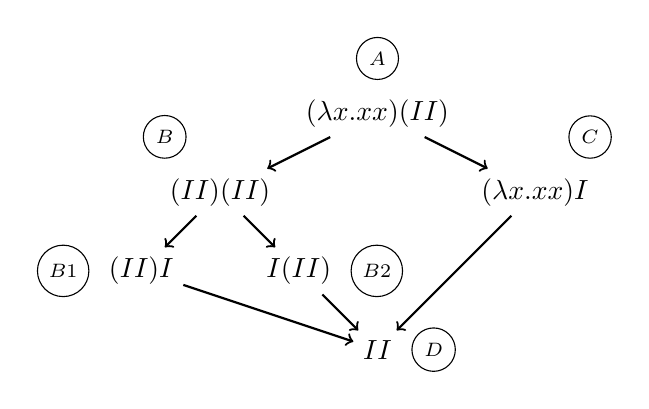
\begin{tikzpicture}[->, every edge/.style={draw=black,thick}]
		\node[label={\scriptsize\tikz\node[circle,draw]{$A$};}]     at (0,   0) (A)  {$(\lambda x . x x)(\comb I \comb I)$};
		\node[label={135:\scriptsize\tikz\node[circle,draw]{$B$};}] at (-2, -1) (B)  {$(\comb I \comb I)(\comb I \comb I)$};
		\node[label={45:\scriptsize\tikz\node[circle,draw]{$C$};}]  at (2,  -1) (C)  {$(\lambda x . x x)  \comb I$};
		\node[label={180:\scriptsize\tikz\node[circle,draw]{$B1$};}]                                                       at (-3, -2) (B1) {$(\comb I \comb I)\comb I$};
		\node[label={0:\scriptsize\tikz\node[circle,draw]{$B2$};}]                                                       at (-1, -2) (B2) {$\comb I(\comb I \comb I)$};
		\node[label={0:\scriptsize\tikz\node[circle,draw]{$D$};}]                                                       at (0,  -3) (D)  {$\comb I \comb I$};
		\path (A)  edge (B)
		edge (C)
		(B)  edge (B1)
		edge (B2)
		(B1) edge (D)
		(B2) edge (D)
		(C)  edge (D);
		\end{tikzpicture}
		\caption{Нет такого $D$, что $B \to_{\beta} D$ и $C \to_{\beta} D$.}
	\end{figure}	
	\\
\end{proof}


\newcommand{\bpar}{\rightrightarrows_{\beta}}

\begin{definition}[Параллельная $\beta$-редукция]
	$A\bpar B$, если
	\begin{enumerate}
		\item $A=_{\alpha}B$
		\item $A\equiv{}P_{1}Q_{1}$, $B\equiv{}P_{2}Q_{2}$ и $P_{1}\bpar P_{2}$, $Q_{1}\bpar Q_{2}$
		\item $A\equiv{}\lambda{}x.P_{1}$, $B\equiv{}\lambda{}x.P_{2}$ и 
		$P_{1}\bpar P_{2}$
		\item $A=_{\alpha}(\lambda{}x.P_1)Q_1$, $B=_{\alpha}P_2[x\coloneqq{}Q_2]$ причем $Q_2$ свободна для подстановки вместо $x$ в $P_2$ и $P_1 \bpar P_2$, $Q_1 \bpar Q_2$
	\end{enumerate}
\end{definition}

\begin{lemma}
	\label{bparhelp}
	Если $P_{1}\bpar P_{2}$ и $Q_{1}\bpar Q_{2}$, то $P_{1}[x\coloneqq{}Q_{1}]\bpar P_{2}[x\coloneqq{}Q_{2}]$
\end{lemma}

\begin{proof}
	Будем доказывать индукцией по определению $\bpar $. Рассмотрим случаи:
	\begin{itemize}
		\item Пусть $P_{1}=_{\alpha}P_{2}$. Тогда лемма легко доказывается индукцией по структуре выражения.
		\item Пусть $P_{1}\equiv{}A_{1}B_{1}$, $P_{2}\equiv{}A_{2}B_{2}$. По определению $(\bpar)$ $A_{1} \bpar A_{2}$ и $B_{1} \bpar B_{2}$.
		Рассмотрим два случая:
		\begin{enumerate}
			\item $x \in \FV(A_{1})$. По индукционному предположению $A_{1}[x\coloneqq{}Q_{1}] \bpar A_{2}[x\coloneqq{}Q_{2}]$. Тогда $A_{1}[x\coloneqq{}Q_{1}]B_{1} \bpar A_{2}[x\coloneqq{}Q_{2}]B_{2}$. Тогда $A_{1}B_{1}[x\coloneqq{}Q_{1}] \bpar A_{2}B_{2}[x\coloneqq{}Q_{2}]$.
			\item $x \in \FV(B_{1})$. По индукционному предположению $B_{1}[x\coloneqq{}Q_{1}] \bpar B_{2}[x\coloneqq{}Q_{2}]$. Тогда $A_{1}B_{1}[x\coloneqq{}Q_{1}] \bpar A_{2}B_{2}[x\coloneqq{}Q_{2}]$.
		\end{enumerate}
		\item Пусть $P_{1}\equiv{}\lambda{}y.A_{1}$, $P_{2}\equiv{}\lambda{}y.A_{2}$. По определению $(\bpar)$ $A_{1}\bpar A_{2}$. Тогда по индукционному предположению $A_{1}[x\coloneqq{}Q_{1}] \bpar A_{2}[x\coloneqq{}Q_{2}]$. Тогда 
		$\lambda{}y.(A_{1}[x\coloneqq{}Q_{1}]) \bpar \lambda{}y.(A_{2}[x\coloneqq{}Q_{2}])$ по определению $(\bpar)$. Следовательно 	$\lambda{}y.A_{1}[x\coloneqq{}Q_{1}] \bpar \lambda{}y.A_{2}[x\coloneqq{}Q_{2}]$ по определению подстановки.
		\item Пусть $P_{1}=_\alpha(\lambda{}y.A_1)B_1$, $P_{2}=_\alpha A_2[y\coloneqq{}B_2]$ и $ A_1 \bpar A_2 $, $ B_1 \bpar B_2 $. По индукционному предположению получаем, что $A_1[x \coloneqq Q_1] \bpar A_2[x \coloneqq Q_2]$, $B_1[x \coloneqq Q_1] \bpar B_2[x \coloneqq Q_2]$. Следовательно, по определению $(\bpar)$ получаем, что $ (\lambda{}y.A_1[x\coloneqq Q_1])B_1[x \coloneqq Q_1] \bpar  A_2[y \coloneqq B_2][x \coloneqq Q_2]$
	\end{itemize}
\end{proof}

\begin{lemma}
	$(\bpar)$ обладает ромбовидным свойством.
\end{lemma}

\begin{proof}
	Будем доказывать индукцией по определению $(\bpar)$. Покажем, что если $M \bpar M_1$ и $M \bpar M_2$, то существует ${}M_3$, что $M_1 \bpar M_3$ и $M_2 \bpar M_3$. Рассмотрим случаи:
	\begin{itemize}
		\item Если $M\equiv M_1$, то просто возьмем $M_3\equiv M_2$.
		\item Если $M\equiv \lambda{}x.P, M_1 \equiv \lambda{}x.P_1, M_2 \equiv \lambda{}x.P_2$ и $P \bpar P_1, P \bpar P_2$, то по предположению индукции 
		существует $P_3$, что $P_1 \bpar P_3, P_2 \bpar P_3$, тогда возьмем $M_3\equiv \lambda{}x.P_3$.
		\item Если $M \equiv P Q, M_1 \equiv P_1 Q_1$ и по определению $(\bpar)$ $P \bpar P_1, Q \bpar Q_1$, то рассмотрим два случая:
		\begin{enumerate}
			\item $M_2 \equiv P_2 Q_2$. Тогда по предположению индукции существует $P_3$, что $P_1 \bpar P_3, P_2 \bpar P_3$. Аналогично для $Q$. Тогда возьмем $M_3 \equiv P_3 Q_3$.
			\item $P\equiv \lambda {}x.P'$ значит $P_1 \equiv \lambda{}x.P_1'$ и $ P' \bpar P_1'$. Пусть тогда $ M_2 \equiv P_2[x\coloneqq{} Q_2]$, по определению $(\bpar)$ $P' \bpar P_2, Q \bpar Q_2$. Тогда по предположению индукции и лемме $\ref{bparhelp}$ существует $M_3 \equiv P_3[x \coloneqq Q_3]$ такой, что $ P_1' \bpar P_3 $, $ Q_1 \bpar Q_3 $ и $ P_2 \bpar P_3 $, $ Q_2 \bpar Q_3 $.
		\end{enumerate}
	\item Если $ M \equiv (\lambda{}x.P)Q $, $ M_1 \equiv P_1[x\coloneqq Q_1] $ и $ P \bpar P_1 $, $ Q \bpar Q_1$, то рассмотрим случаи:
	\begin{enumerate}
		\item $ M_2 \equiv (\lambda{}x.P_2)Q_2 $, $P \bpar P_2$, $Q \bpar Q_2$. Тогда по предположению индукции и лемме $ \ref{bparhelp} $ существует такой $ M_3 \equiv P_3[x \coloneqq Q_3] $, что $ P_1 \bpar P_3 $, $ Q_1 \bpar Q_3 $ и $ P_2 \bpar P_3 $, $ Q_2 \bpar Q_3 $.
		\item $ M_2 \equiv P_2[x \coloneqq Q_2]$, $ P \bpar P_2 $, $ Q \bpar Q_2 $. Тогда по предположению индукции и лемме $ \ref{bparhelp} $ существует такой $ M_3 \equiv P_3[x \coloneqq Q_3] $, что $ P_1 \bpar P_3 $, $ Q_1 \bpar Q_3 $ и $ P_2 \bpar P_3 $, $ Q_2 \bpar Q_3 $.
	\end{enumerate}
	\end{itemize}
\end{proof}

\begin{lemma}
	\
	\begin{enumerate}
		\item $(\bpar )^{*} \subseteq (\to_{\beta})^{*}$
		\item $(\to_{\beta})^{*} \subseteq (\bpar )^{*}$
	\end{enumerate}
\end{lemma}

\begin{cons}
	$(\to_{\beta})^{*}=(\bpar )^{*}$
\end{cons}

Из приведенных выше лемм и следствия докажем теорему Черча-Россера.

\begin{proof}
	$(\to_{\beta})^{*} = (\twoheadrightarrow_{\beta})$. Тогда $(\twoheadrightarrow_{\beta})=(\bpar )^{*}$. Значит из того, что $(\bpar )$ обладает ромбовидным свойством и леммы $\ref{refl}$, следует, что $(\twoheadrightarrow_{\beta})$ обладает ромбовидным свойством.
\end{proof}

\subsection{Нормальный и аппликативный порядок вычислений}

\begin{example}
	Выражение $KI\Omega$ можно редуцировать двумя способами:
	\begin{enumerate}
		\item $\comb K \comb I \Omega =_{\alpha} ((\lambda{}a.\lambda{}b.a) \comb I) \Omega \to_{\beta} (\lambda{}b.\comb I)\Omega  \to_{\beta} \comb I$
		\item  $\comb K \comb I \Omega =_{\alpha} ((\lambda{}a.\lambda{}b.a) \comb I)((\lambda{}x.x \ x) (\lambda{}x.x \ x)) \twoheadrightarrow_{\beta} ((\lambda{}a.\lambda{}b.a) \comb I)((\lambda{}x.x \ x) (\lambda{}x.x \ x)) \to_{\beta} \comb K \comb I \Omega $
	\end{enumerate}
	
\end{example}

Как мы видим, в первом случае мы достигли нормальной формы, в то время как во втором мы получили бесконечную редукцию. Разница двух этих способов в порядке редукции. Первый называется нормальный порядок, а второй аппликативный. 

\begin{definition}[нормальный порядок редукции]
	Редукция самого левого $\beta$-редекса.
\end{definition}

\begin{definition}[аппликативный порядок редукции]
	Редукция самого левого $\beta$-редекса из самых вложенных.
\end{definition}

\begin{theorem}[Приводится без доказательства]
	Если нормальная форма существует, она может быть достигнута нормальным порядком редукции.
\end{theorem}

Нормальный порядок хоть и приводит к нормальной форме, если она существует, но бывают ситуации, в которых аппликативный порядок вычисляется быстрее, чем нормальный.

\begin{example}
	Рассмотрим $\lambda$-выражение $(\lambda{}x.x \ x \ x \ x) (\comb I \comb I)$. Попробуем редуцировать его нормальным порядком:
	 \[(\lambda{}x.x \ x \ x \ x) (\comb I \comb I) \to_{\beta} (\comb I \comb I)(\comb I \comb I)(\comb I \comb I)(\comb I \comb I) \to_{\beta} \comb I(\comb I \comb I)(\comb I \comb I)(\comb I \comb I) \to_{\beta} (\comb I \comb I)(\comb I \comb I)(\comb I \comb I) \to_{\beta} \ldots \to_{\beta} \comb I\] 
	Как мы увидим, в данной ситуации аппликативный порядок редукции оказывается значительно эффективней: 
	\[ (\lambda{}x.x \ x \ x \ x) (\comb I \comb I) \to_{\beta} (\lambda{}x.x \ x \ x \ x) \comb I \to_{\beta} \comb I \comb I \comb I \comb I\to_{\beta} \comb I \comb I \comb I \to_{\beta} \comb I \comb I \to_{\beta} \comb I \]
\end{example}
